\documentclass[notitlepage,aps,prd,nofootinbib]{revtex4-1}

\usepackage{subfig}
%\usepackage[colorinlistoftodos]{todonotes}
\usepackage{float}

%\usepackage[protrusion=true,expansion=true]{microtype}
\usepackage{amsmath}
\usepackage{amssymb}
\usepackage{bbm}
\usepackage{ulem}
%\usepackage{feynmp-auto}
%\usepackage{slashed}
%\usepackage[absolute,overlay]{textpos}
\usepackage[usenames, dvipsnames]{color}
\usepackage{graphicx}
\usepackage{listings}
\usepackage{epsfig}
\usepackage{hyperref}
%\usepackage{tikz}
\usepackage{enumerate}
%\usepackage{fixltx2e} % buggy
\usepackage[compatibility=false]{caption}
%\usepackage{subcaption} % doesn't work with subfigure
\usepackage{pdfpages}
%\usepackage{setspace}
\usepackage{verbatim}

% Turn off meaningless float warnings
\usepackage{silence}
\WarningFilter{revtex4-1}{Repair the float}

\DeclareRobustCommand{\orderof}{\ensuremath{\mathcal{O}}}

\definecolor{dukeblue}{RGB}{0,0,156}
\definecolor{dukedarkblue}{RGB}{0,26,87}
\definecolor{dukeblack}{RGB}{79,79,79}
\definecolor{dukegray}{RGB}{79,79,79}
\definecolor{dukesecbrown}{RGB}{217,200,158}
\definecolor{dukesecblue}{RGB}{127,169,174}

%\renewcommand*{\thefootnote}{\fnsymbol{footnote}}

%%%%%%%%%%%%%%%%%%%%%%%%%%%%%%%%%%%%%%%%%%%%%%%%%%%%%%%%%%%%%%%%%%%%%%%%%%%%%%%%%%%%%
\hypersetup{
    breaklinks,
    baseurl       = http://,
    pdfborder     = 0 0 0,
    pdfpagemode   = UseNone,% do not show thumbnails or bookmarks on opening
    pdfstartpage  = 1,
    bookmarksopen = true,
    bookmarksdepth= 2,% to show sections and subsections
% revtex needs author and title declared after \begin{document}, so have to hard code them...
%    pdfauthor     = {\@author},
%    pdftitle      = {\@title},
    pdfauthor     = {Matthew Epland},
    pdftitle      = {Phys 566 HW4},
    pdfsubject    = {},
    pdfkeywords   = {}}


% Code import settings
%%%%%%%%%%%%%%%%%%%%%%%%%%%%%%%%%%%%%%%%%%%%%%%%%%%%%%%%%%%%%%%%%%%%%%%%%%%%%%%%%%%%%
\definecolor{mygreen}{rgb}{0,0.6,0}
\definecolor{mygray}{rgb}{0.5,0.5,0.5}
\definecolor{mymauve}{rgb}{0.58,0,0.82}

%\lstset{ %
\lstdefinestyle{python}{ %
  backgroundcolor=\color{white},   % choose the background color; you must add \usepackage{color} or \usepackage{xcolor}
  basicstyle=\scriptsize,          % the size of the fonts that are used for the code
  breakatwhitespace=false,         % sets if automatic breaks should only happen at whitespace
  breaklines=true,                 % sets automatic line breaking
  captionpos=b,                    % sets the caption-position to bottom
  commentstyle=\color{mygreen},    % comment style
  deletekeywords={...},            % if you want to delete keywords from the given language
  escapeinside={\%*}{*)},          % if you want to add LaTeX within your code
  extendedchars=true,              % lets you use non-ASCII characters; for 8-bits encodings only, does not work with UTF-8
  frame=single,	                   % adds a frame around the code
  keepspaces=true,                 % keeps spaces in text, useful for keeping indentation of code (possibly needs columns=flexible)
  keywordstyle=\color{blue},       % keyword style
  language=Python,                 % the language of the code
  otherkeywords={*,...},           % if you want to add more keywords to the set
  numbers=left,                    % where to put the line-numbers; possible values are (none, left, right)
  numbersep=5pt,                   % how far the line-numbers are from the code
  numberstyle=\tiny\color{mygray}, % the style that is used for the line-numbers
  rulecolor=\color{black},         % if not set, the frame-color may be changed on line-breaks within not-black text (e.g. comments (green here))
  showspaces=false,                % show spaces everywhere adding particular underscores; it overrides 'showstringspaces'
  showstringspaces=false,          % underline spaces within strings only
  showtabs=false,                  % show tabs within strings adding particular underscores
  stepnumber=5,                    % the step between two line-numbers. If it's 1, each line will be numbered
  stringstyle=\color{mymauve},     % string literal style
  tabsize=2,	                   % sets default tabsize to 2 spaces
%  title=\lstname                   % show the filename of files included with \lstinputlisting; also try caption instead of title
  title={\protect\filename@parse{\lstname}\protect\filename@base.\filename@ext},
  firstnumber=0,
%  linewidth=0.95\textwidth
  xleftmargin=0.01\textwidth,
  xrightmargin=0.01\textwidth
}

\lstdefinestyle{output}{ %
  backgroundcolor=\color{white},   % choose the background color; you must add \usepackage{color} or \usepackage{xcolor}
  basicstyle=\scriptsize,          % the size of the fonts that are used for the code
  breakatwhitespace=false,         % sets if automatic breaks should only happen at whitespace
  breaklines=true,                 % sets automatic line breaking
  captionpos=b,                    % sets the caption-position to bottom
  escapeinside={\%*}{*)},          % if you want to add LaTeX within your code
  frame=single,	                   % adds a frame around the code
  keepspaces=true,                 % keeps spaces in text, useful for keeping indentation of code (possibly needs columns=flexible)
  numbers=left,                    % where to put the line-numbers; possible values are (none, left, right)
  numbersep=5pt,                   % how far the line-numbers are from the code
  numberstyle=\tiny\color{mygray}, % the style that is used for the line-numbers
  rulecolor=\color{black},         % if not set, the frame-color may be changed on line-breaks within not-black text (e.g. comments (green here))
  stepnumber=5,                    % the step between two line-numbers. If it's 1, each line will be numbered
  tabsize=2,	                   % sets default tabsize to 2 spaces
%  title=\lstname                   % show the filename of files included with \lstinputlisting; also try caption instead of title
  title={\protect\filename@parse{\lstname}\protect\filename@base.\filename@ext},
  firstnumber=0,
%  linewidth=0.95\textwidth
  xleftmargin=0.01\textwidth,
  xrightmargin=0.01\textwidth
}

\newcommand{\degree}{\ensuremath{^{\circ}}}

% TODO
% Select between raw and saved plots here
\graphicspath{{../code/output/}} % raw plots
%\graphicspath{{./output/}} % saved plots

%%%%%%%%%%%%%%%%%%%%%%%%%%%%%%%%%%%%%%%%%%%%%%%%%%%%%%%%%%%%%%%%%%%%%%%%%%%%%%%%%%%%%
\begin{document}

\title{PHYS 566 HW4}
\author{Matthew Epland}
\affiliation{Department of Physics, Duke University, Durham, NC 27707, USA}

\date{\today}

\begin{abstract}
TODO

\end{abstract}\maketitle


\section{Introduction}
\label{sec:intro}
TODO

\section{Theory}
\label{sec:theory}
The equation of motion of a damped, driven pendulum (\ref{eq:diff_eq}) is a TODO second order linear equation. As written all of the constants are positive real numbers. It is helpful to rewrite (\ref{eq:diff_eq}) as (\ref{eq:diff_eq2}) where $\omega_{0}^2 = \frac{g}{l}$ and $F\left(t\right)$ is the external driving force.

\begin{equation} \label{eq:diff_eq}
\frac{d^2 \theta}{d t^2} = -\frac{g}{l}\theta - 2\gamma\frac{d \theta}{d t} + \alpha_{D}\sin\left(\Omega_{D} t\right)
\end{equation}

\begin{equation} \label{eq:diff_eq2} 
\begin{gathered}
\ddot{\theta} + 2\gamma \dot{\theta} + \omega_{0}^2 \theta = F\left(t\right) \\
F\left(t\right) = \alpha_{D} \sin\left(\Omega_{D} t\right)
\end{gathered}
\end{equation}

The solution to (\ref{eq:diff_eq2}) can be broken into two parts, the solution of the associated homogeneous equation where $F\left(t\right) = 0$ and any particular solution of (\ref{eq:diff_eq2}). To begin with we will solve the homogeneous equation by assuming a solution of the form $\theta\left(t\right) \sim e^{r t}$, which is indeed a solution provided that $r$ is a root of the characteristic equation (\ref{eq:characteristic_eq}). Using the quadratic formula we find the two roots to be $r_{\pm}$ (\ref{eq:r_pm}), thereby specifying the homogeneous solution\footnote{If $\gamma = \omega_{0}$, and therefore $r_{+} = r_{-}$, we need to include a multiplicative factor of $t$ on one of the solutions so that they are linearly independent.} (\ref{eq:homogeneous_soln}). 

\begin{gather}
r^2 + 2 \gamma r + \omega_{0}^2 = 0 \label{eq:characteristic_eq} \\
r_{\pm} = -\gamma \pm \sqrt{\gamma^2 - \omega_{0}^2} \label{eq:r_pm}
\end{gather}

\begin{equation} \label{eq:homogeneous_soln}
\theta\left(t\right)_{\text{homogeneous}} =
\begin{cases}
A e^{r_{+} t} + B e^{r_{-} t} & \text{if } \gamma \neq \omega_{0} \\
\left(A + B t\right) e^{-\gamma t} & \text{if } \gamma = \omega_{0}
\end{cases}
\end{equation}

It is easy to see from (\ref{eq:r_pm}) that $\operatorname{Re}\left(r_{\pm}\right) < 0$ for all $\gamma$ and $\omega_{0}$, therefore the homogeneous solution (\ref{eq:homogeneous_soln}) always decays away to nothing; it is a transient solution. As we are primary interested in the steady state behavior of the pendulum in this assignment, we therefore need only be concerned with the particular solution from here on out.

We can find a particular solution (\ref{eq:particular_soln}) that works by trial and error. Plugging (\ref{eq:particular_soln}) into (\ref{eq:diff_eq2}) with $F\left(t\right) \neq 0$ results in (\ref{eq:part_work}).

\begin{equation} \label{eq:particular_soln}
\theta\left(t\right)_{\text{particular}} = \theta_{0} \sin\left(\Omega_{D} t - \phi\right)
\end{equation}

\begin{equation} \label{eq:part_work}
TODO
\end{equation}

\begin{equation} \label{eq:trig_identity}
\sin\left(\alpha + \beta\right) = \sin\left(\alpha\right) \cos\left(\beta\right) + \cos\left(\alpha\right) \sin\left(\beta\right)
\end{equation}


\subsection{Resonance}
\label{subsec:resonance}
TODO

\subsection{Euler--Cromer}
\label{subsec:eulercromer}
In the past we have used the Euler method solve differential equations time step to time step. The advantage of using the Euler method is its simplicity, however its solutions usually do not conserve energy but increase in total energy over time. We can remedy this by switching to the Euler--Cromer method, also known as the semi-implicit Euler method\footnote{The name semi-implicit comes from the fact that $n+1$ data in the form of $\omega_{n+1}$ is being used to compute $\theta_{n+1}$. Also note that like the unmodified Euler method, the Euler--Cromer method is still only a TODO $\orderof\big(\left(\Delta t\right)^2\big)$ method.}, by modifying the Euler method to use $\omega_{n+1}$ instead of $\omega_{n}$ when computing $\theta_{n+1}$, see (\ref{eq:euler_chromer1}, \ref{eq:euler_chromer2}).

\begin{align}
\frac{d \theta}{d t} &= f\left(t, \omega\right) &
\frac{d \omega}{d t} &= \frac{d^2 \theta}{d t^2} = g\left(t, \theta\right) \label{eq:euler_chromer1} \\
\omega_{n+1} &= \omega_{n} + g\left(t_{n}, \theta_{n};~\omega_{n}\right) \Delta t & 
\theta_{n+1} &= \theta_{n} + f\left(t_{n}, \underline{\omega_{n+1}}\right) \Delta t \label{eq:euler_chromer2}
\end{align}

Applying the Euler--Cromer method to our pendulum problem, we have:

\begin{align} \label{eq:euler_chromer_applied}
\omega_{n+1} &= \omega_{n} + \bigg( -\frac{g}{l}\theta_{n} - 2\gamma \omega_{n} + \alpha_{D}\sin\left(\Omega_{D} t_{n}\right) \bigg) \Delta t \\
\theta_{n+1} &= \theta_{n} + \omega_{n+1} \Delta t \\
t_{n} &= t_{0} + n \Delta t = n \Delta t
\end{align}


\subsection{Runge--Kutta}
\label{subsec:runge_kutta}
TODO
Runge--Kutta method


\clearpage
\section{Results}
\label{sec:results}
TODO


\begin{comment}
\begin{figure}[!htbc]
  \centering
  \includegraphics[width=.7\textwidth]{}
	{\par\nobreak\rule[9pt]{35em}{0.5pt}\vspace{-5mm}}
	\caption{}
	\label{fig:}
\end{figure}
\end{comment}

\section{Conclusions}
\label{sec:Conclusions}
TODO

The Python source code used to produce these results can be found online at \url{http://github.com/mepland/PHYS_566_Computational_HW/tree/master/hw4/code}, and is included in Section~\ref{sec:code}.

\clearpage
\section{Supporting Material}
\label{sec:Supporting_Material}

% TODO
%\lstinputlisting[style=output,label={lst:output}]{../code/output.log} % raw
%\lstinputlisting[style=output,label={lst:output}]{./output/output.log} % saved 

\clearpage
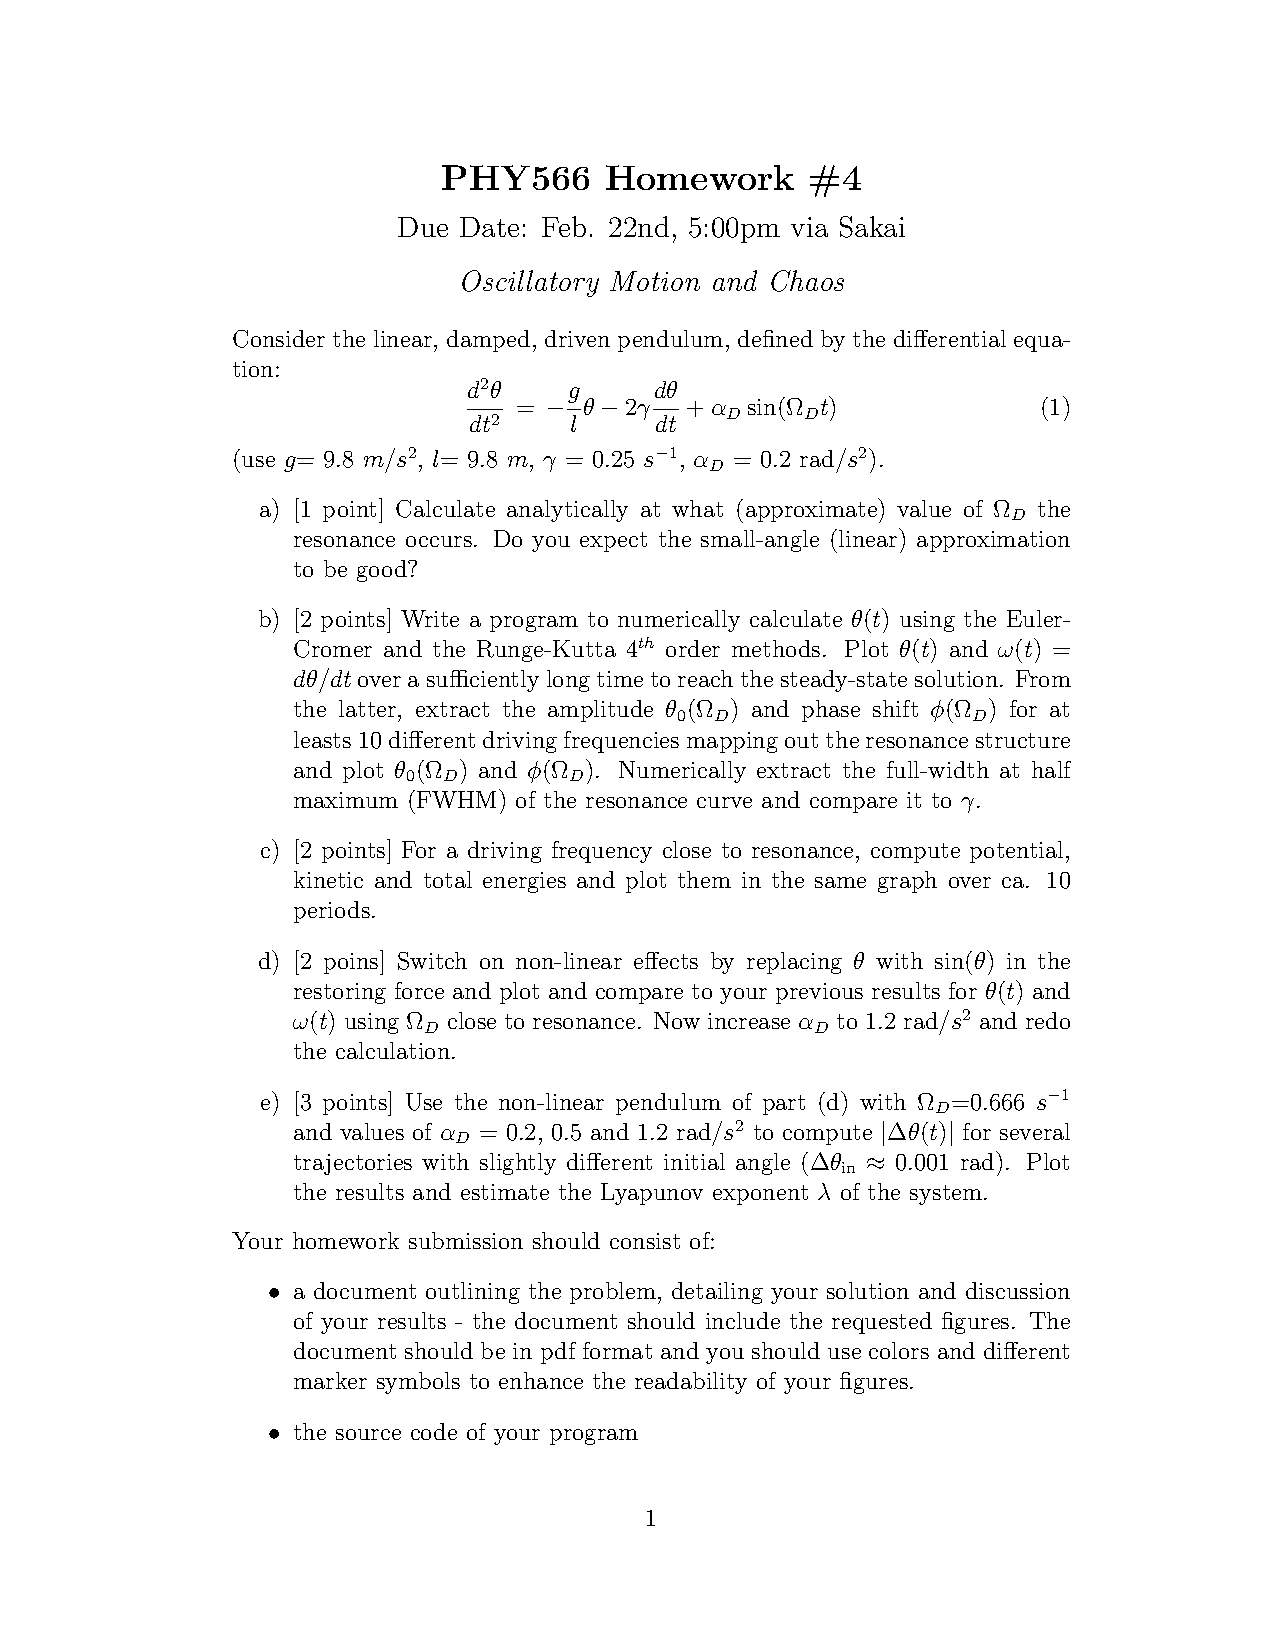
\includepdf{../homework4.pdf}

\clearpage
\section{Code}
\label{sec:code}

%TODO add more if there are multiple .py's
\lstinputlisting[style=python]{../code/chaotic_pendulum.py}

\end{document} %%% end of doc %%%
%%%%%%%%%%%%%%%%%%%%%%%%%%%%%%%%%%%%%%%%%%%%%%%%%%%%%


\bibliographystyle{bib_files/styles/atlasBibStyleWoTitle}
\bibliography{bib_files/my_bib.bib}


